\section{Servicemodelle}

\subsection{Infrastructure as a Service (IaaS)}
Bei \textbf{IaaS} wird dem Nutzer \emph{ausschließlich die Infrastruktur} bereitgestellt.
Ein typisches Beispiel sind virtuelle Maschinen. Der Nutzer ist selbst für
das Betriebssystem und alle darauf installierten Anwendungen verantwortlich.
\textit{Load Balancer} und ähnliche Dienste sind nicht vorkonfiguriert und müssen
manuell eingerichtet werden.

\textbf{Flexibilität:} Hoch, man ist bei der Nutzung vollständig frei.\\
\textbf{Verantwortung:} Hoch, nur die physische Hardware muss nicht selbst
verwaltet werden.\\
\textbf{Typische Anwendungsfälle:} Entwicklungs-Workloads und Hosten von
Legacy-Systemen.
\begin{table}[h]
    \centering
    \begin{tabularx}{\linewidth}{|X|X|X|}
        \hline
        \textbf{Public Cloud} & \textbf{Private Cloud} & \textbf{Hybrid Cloud} \\
        \hline
        IaaS in der Public Cloud wird oft genutzt, um virtuelle Server bereitzustellen, insbesondere für Startups. Zusätzlich ist IaaS in der Public Cloud kostengünstig und skalierbar. & Große Unternehmen können IaaS auch in ihrer Private Cloud nutzen, um maximale Kontrolle über Computing-Ressourcen zu haben. & Die meiste Rechenleistung befindet sich in der Private Cloud, nur bei Spitzenlasten wird auf die Public Cloud gewechselt. Auch Cloud Bursting genannt. \\
        \hline
    \end{tabularx}
\end{table}
\subsection{Platform as a Service (PaaS)}
Bei \textbf{PaaS} bewegt man sich in Richtung \textit{Managed Services}. Ein Beispiel wäre
eine verwaltete SQL-Datenbank in Azure. Viele Aspekte wie Load Balancer und
Skalierung werden bereits vom Anbieter übernommen, was die Entwicklung
deutlich vereinfacht.

\textbf{Flexibilität:} Hoch, allerdings mit deutlich weniger
Konfigurationsaufwand als bei IaaS.\\
\textbf{Verantwortung:} Mittel, viele Dienste werden bereits vom Provider
verwaltet.\\
\textbf{Typische Anwendungsfälle:} Hosten von Webanwendungen, verwaltete
Datenbanken in der Cloud.
\begin{table}[h]
    \centering
    \begin{tabularx}{\linewidth}{|X|X|X|}
        \hline
        \textbf{Public Cloud} & \textbf{Private Cloud} & \textbf{Hybrid Cloud} \\
        \hline
        PaaS wird in der Public Cloud genutzt, um Anwendungen von Entwicklern bereitzustellen. Beispielsweise soll eine Webanwendung für das ganze Unternehmen zur Verfügung gestellt werden – dies wird in Azure beispielsweise über einen Azure App Service getan. & PaaS-Plattformen können auch in einem unternehmenseigenen Rechenzentrum eingerichtet werden, sodass Entwicklungsteams in einer sicheren Umgebung testen können. & Entwicklungsteams testen in einer privaten PaaS-Umgebung und deployen die Anwendung dann in eine öffentliche PaaS-Umgebung. \\
        \hline
    \end{tabularx}
\end{table}
\subsection{Software as a Service (SaaS)}
Bei \textbf{SaaS} erhält der Nutzer ein \emph{fertiges Produkt}, das nur noch konfiguriert
werden muss. Eigener Code kann nicht eingebunden werden, alles funktioniert
über \textit{Customizing}.

\textbf{Flexibilität:} Gering, alles skaliert automatisch, eigene Eingriffe
sind kaum möglich.\\
\textbf{Verantwortung:} Gering, der Nutzer ist nur für die eigenen Daten
verantwortlich.\\
\textbf{Typische Anwendungsfälle:} Produkte wie Microsoft 365.
\begin{table}[h]
    \centering
    \begin{tabularx}{\linewidth}{|X|X|X|}
        \hline
        \textbf{Public Cloud} & \textbf{Private Cloud} & \textbf{Hybrid Cloud} \\
        \hline
        SaaS-Produkte wie Microsoft 365, Gmail oder Salesforce sind am weitesten verbreitet. Eine Anwendung läuft komplett in der Public-Cloud-Infrastruktur eines Anbieters. Die Anwendungen werden über das Internet bereitgestellt. & SaaS-Produkte können bei Unternehmen mit hohen Sicherheitsanforderungen in der eigenen Cloud-Infrastruktur gehostet werden. Beispielsweise können auch KI-Modelle wie Claude oder Gemini bei einem Unternehmen selbst gehostet werden. & Dies ist eine häufige Kombination in Unternehmen: Sensible Daten liegen On-Premises in der Private Cloud, beispielsweise auch ein ERP-System. Daneben werden aber auch SaaS-Anwendungen wie Teams oder Gmail genutzt. \\
        \hline
    \end{tabularx}
\end{table}
\newpage
\subsection{Shared Responsibility Model}
Das \textbf{Shared Responsibility Model} zeigt auf, wo die Verantwortlichkeiten bei
Cloud-Modellen liegen und wie viel vom Nutzer bzw. Unternehmen selbst
gemanagt werden muss im Vergleich zu dem, was der Cloud-Provider übernimmt.

\begin{figure}[H]
    \centering
    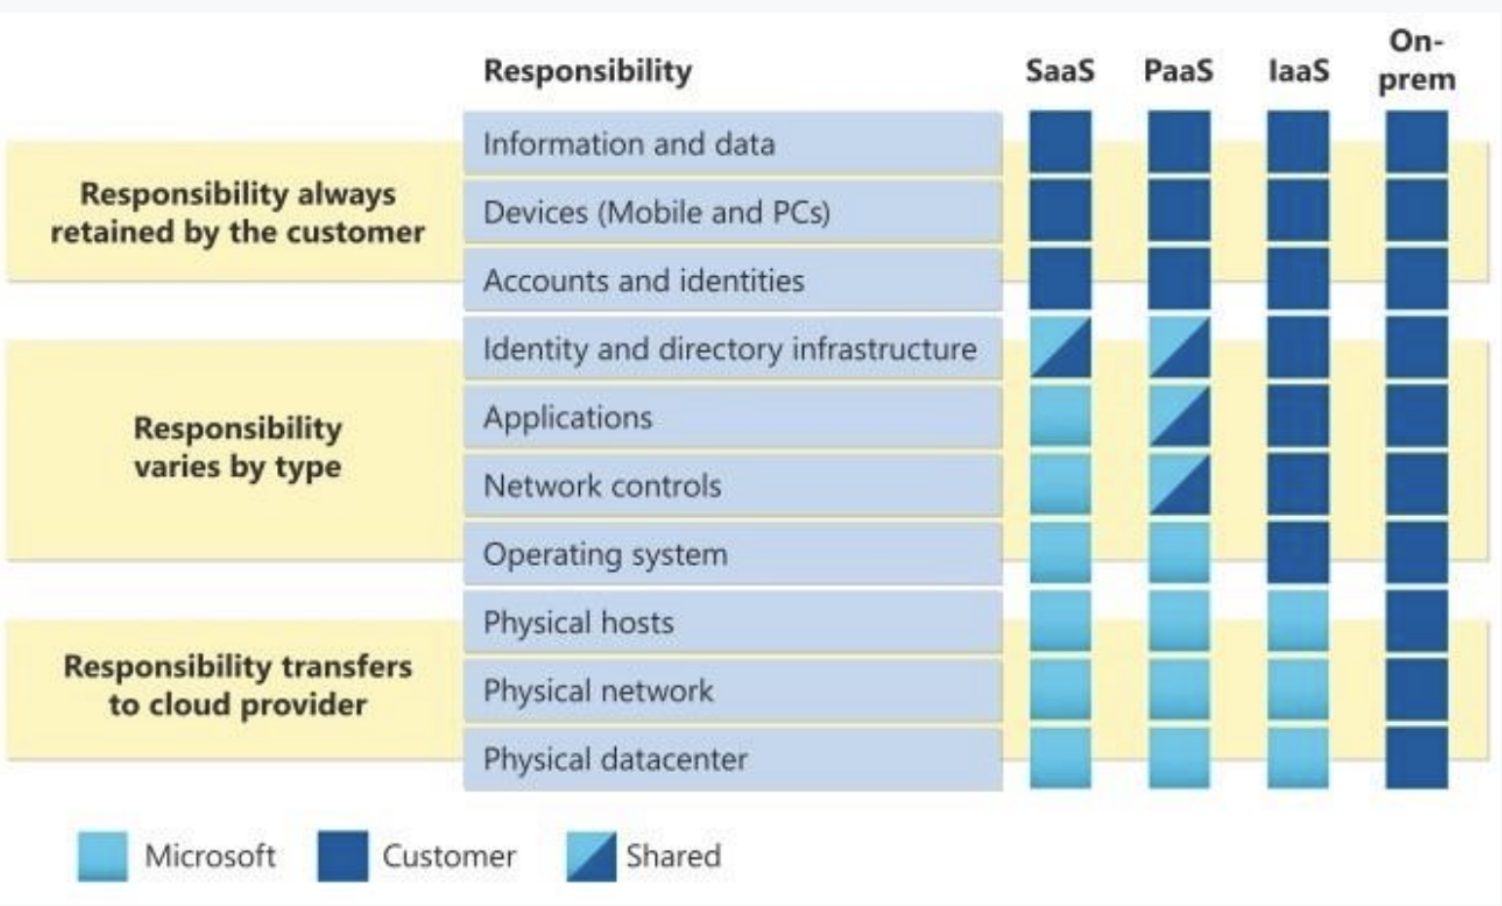
\includegraphics[width=\textwidth]{assets/images/SharedResponbility}
    \caption{Shared Responsibility Model}
\end{figure}

\subsubsection{Sicherheitsaufgaben von Kunde und Provider}
Der Kunde ist hauptsächlich für die Sicherheit der Client-Geräte
verantwortlich, also beispielsweise dafür, dass Mitarbeiter sichere
Passwörter verwenden. Zusätzlich können \textit{RBAC} und \textit{Conditional Access}
aktiviert werden, sodass Endnutzer automatisch mehr Sicherheit erhalten.
Authentifizierung, die beispielsweise \textit{SSO} ermöglicht, wird vom Cloud-Provider
bereitgestellt. Der Provider ist seinerseits vollständig für die Sicherheit
im Rechenzentrum und seiner eigenen Services zuständig. Für die Sicherheit
der eigenen Daten ist der Kunde verantwortlich, muss dafür aber oft nur
wenige Konfigurationen vornehmen, beispielsweise Disaster Recovery durch
Zonenredundanz.

\subsubsection{Warum verändern sich die Verantwortlichkeiten?}
Die verschiedenen Servicemodelle haben unterschiedliche Anwendungsfälle.
IaaS wird genutzt, wenn möglichst viel selbst konfiguriert werden soll,
beispielsweise für das Hosten von Legacy-Systemen oder Entwicklungs-Workloads.
Die Kosten für den Compute werden dabei oft im Voraus bezahlt, beispielsweise
über \textit{Azure Reservations}. PaaS wird für eigene Cloud-Native-Anwendungen
genutzt, hat aber grundlegende Dinge bereits vorkonfiguriert, sodass keine
VM manuell eingerichtet werden muss. SaaS sind vollständig abgeschlossene
Softwareprodukte, die einfach über die Cloud laufen, wie beispielsweise
Microsoft 365.